\chapter{Materiais e Métodos}
\label{ch:metodologia}
\section{Considerações Iniciais}
Neste capítulo apresentam-se a classificação da pesquisa e o plano metodológico adotado para o alcance do objetivo desta pesquisa, isto é: \textit{Obter perfis de testadores utilizando características e experiência do domínio para Atribuição automática de tarefas de teste, utilizando a equipe de transformação de serviços do governo do ITRAC - Information Technology and Application Center}.

Assim, apresenta-se o planejamento metodológico em fases e atividades.Seguido do diagnóstico do objeto de estudo.

\section{Plano Metodológico Adotado}
\label{sec:planMetodologico}

O plano metodológico adotado neste trabalho compreende quatro fases básicas: planejamento da pesquisa; coleta de dados; análise dos dados; e relato dos resultados, como apresentado  na Figura \ref{fig:PlanoGeral} abaixo:

        \begin{figure}[H]
          \centering
          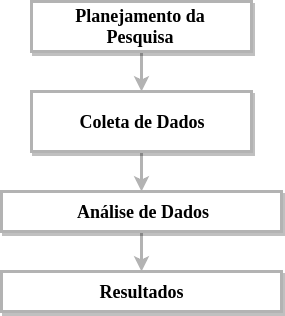
\includegraphics[width=6cm]{figuras/planoGeral.png}
          \caption{Plano metodológico adotado (Fonte: Elaborado pela Autora.)}
          \label{fig:PlanoGeral}

        \end{figure}

O trabalho foi desenvolvido no contexto do laboratório ITRAC, junto ao time de testadores envolvidos nos testes dos serviços transformados para o ME. Sendo assim, o objeto de estudo é o\textit{ time de testadores do ITRAC}.

Na fase de coleta de dados os procedimentos de pesquisa empregados foram: pesquisa documental; pesquisa bibliográfica; e a prototipação. Um questionário foi elaborado para aplicação futura dentre os membros da equipe de teste.

Nas subseções caracterizadas pelas fases do plano metodológico são apresentadas juntamente com uma descrição de cada um dos procedimentos empregados, como apresentado na Figura \ref{fig:fasesPlano}.


        \begin{figure}[H]
          \centering
          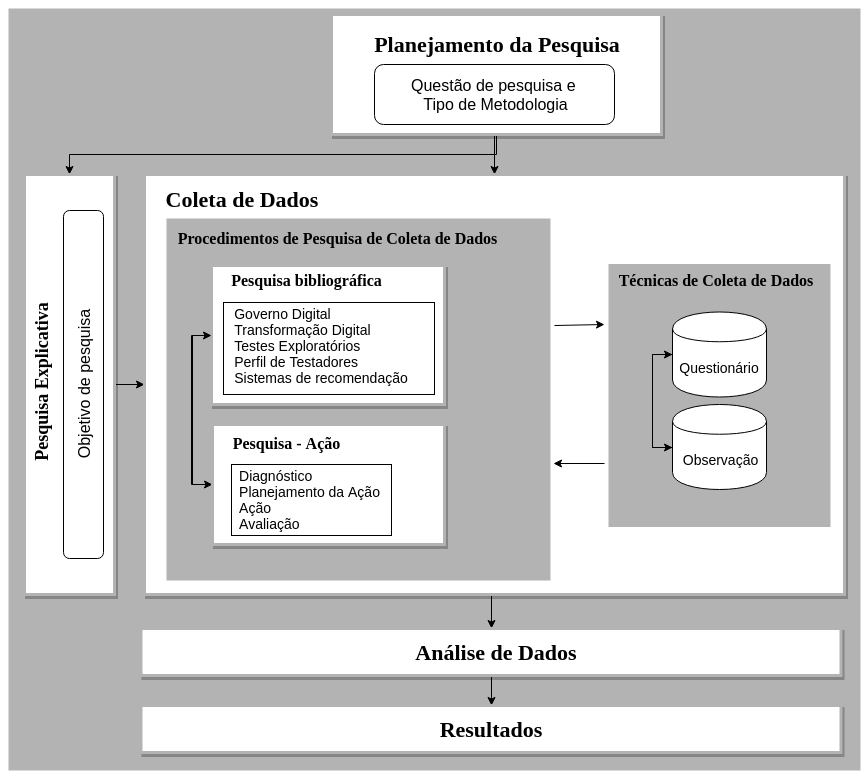
\includegraphics[width=16cm]{figuras/fasesPlanoMetodologico.png}
          \caption{Fases do Plano Metodológico adotadas nesta pesquisa. (Fonte: Elaborado pela Autora.)}
          \label{fig:fasesPlano}

        \end{figure}


\subsection{Fase de Planejamento da Pesquisa}

Na fase de Planejamento da Pesquisa foi configurada a elaboração de todo o Capítulo \ref{ch:introducao} de Introdução. Foi definido o tema de pesquisa, pergunta de pesquisa, objetivos e, também, definição e classificação metodológica.

A Figura \ref{fig:PlanPesquisa} apresenta esta fase importante para as definições iniciais da pesquisa.

        \begin{figure}[H]
          \centering
          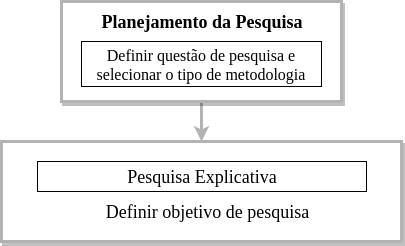
\includegraphics[width=6.5cm]{figuras/planejamentoPesquisa.png}
          \caption{Planejamento da pesquisa. (Fonte: Elaborado pela Autora.)}
          \label{fig:PlanPesquisa}

        \end{figure}


        % \begin{figure}[H]
        %   \centering
        %   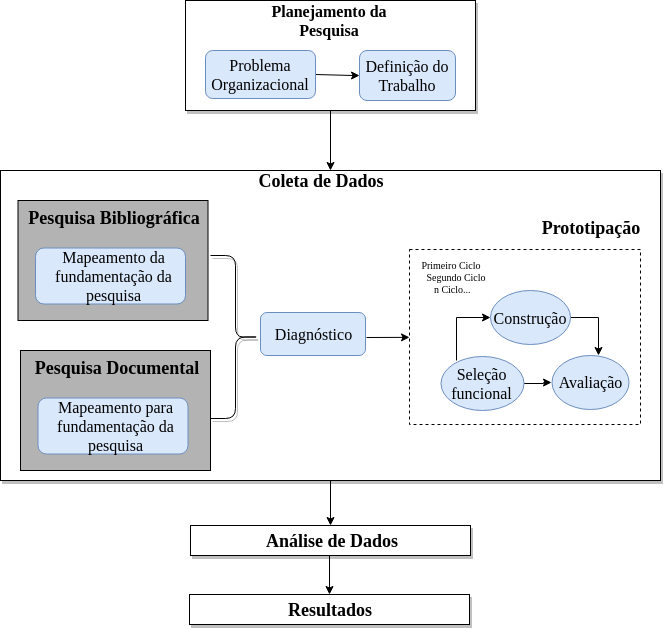
\includegraphics[width=14cm]{figuras/planoMetodologico.png}
        %   \caption{Plano metodológico adotado (Fonte: Elaborado pela Autora.)}
        %   \label{fig:PlanoMetodologico}

        % \end{figure}

\subsection{Fase de Coleta de Dados}

A fase de coleta de dados configurou o recolhimento de boa parte do conteúdo necessário para a consolidação deste trabalho, foram adotados os procedimentos de \textit{pesquisa bibliográfica} e adotados os procedimentos da \textit{pesquisa - ação}.

A Figura \ref{fig:coletaDados} apresenta os procedimentos de coleta de dados e as técnicas adotadas para o presente trabalho.

        \begin{figure}[H]
          \centering
          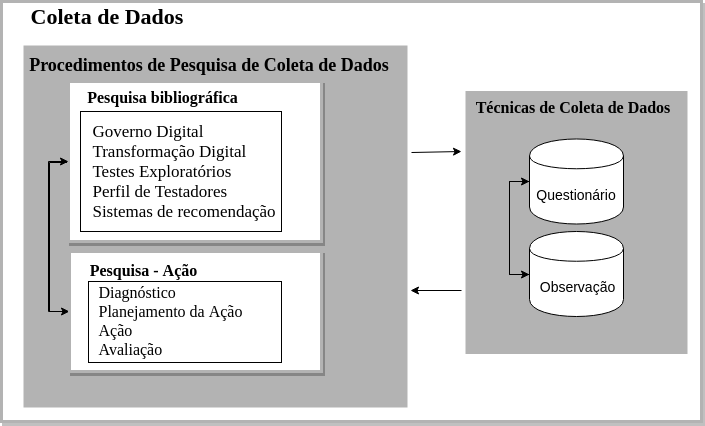
\includegraphics[width=10cm]{figuras/coletadeDados.png}
          \caption{Coleta de Dados. (Fonte: Elaborado pela Autora.)}
          \label{fig:coletaDados}

        \end{figure}

A análise bibliográfica permitiu com que fosse recolhido embasamentos relevantes sobre os temas relacionados a esta pesquisa. Algumas atividades da pesquisa-ação já realizadas também promoveram uma iteração maior entre pesquisados e equipe do objeto de estudo do laboratório.

\subsection{Pesquisa Bibliográfica}

A partir da pesquisa bibliográfica foi possível recolher embasamentos relevantes sobre Governo Digital, Transformação Digital, Testes Exploratórios, Perfil de Testadores e Sistemas de Recomendação. Cada um dos embasamentos sobre os temas coletados foram apresentados no Capítulo \ref{ch:referencial} de Referencial Teórico.

\subsection{Fase de Pesquisa-Ação}
\label{sub:pesquisa-acao}

A estratégia de Pesquisa-Ação neste trabalho foi adotada a partir de uma adaptação da pesquisa-ação proposta por \cite{petersen2008systematic}. Na estratégia são propostas 4 etapas distintas, conforme apresentado na Figura \ref{fig:etapasPesquisaAcao}.

        \begin{figure}[H]
          \centering
          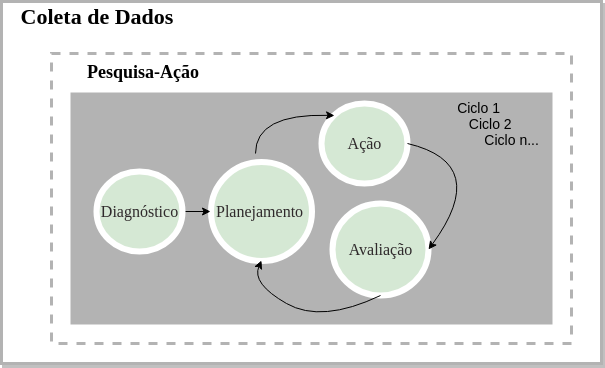
\includegraphics[width=12cm]{figuras/etapasPesquisaAcao.png}
          \caption{Etapas da estratégia de Pesquisa-Ação adotada. (Fonte: Elaborado pela Autora.)}
          \label{fig:etapasPesquisaAcao}

        \end{figure}

É importante ressaltar que a estratégia será empregada em ciclos para a fase de implementação do sistema de recomendação, ou seja, a adaptação da ideia e melhoria da proposta deste trabalho irá permitir uma maior iteração com a equipe de testadores de modo que, de maneira colaborativa, se extraiam mais informações relevantes para a otimização da recomendação realizada pelo sistema.

\subsection{Diagnóstico}

Para a construção do sistema de recomendação um \textit{diagnóstico} foi realizado para a compreensão do objeto de estudo. Para a caracterização do objeto de estudo, apresentado no Capítulo \ref{ch:referencial}, foram realizadas pesquisas quanto a sistemas de recomendação e perfil de testadores, a fim de entender o \textit{background} teórico deste trabalho.

% \del{``afundo'' - vem de afundar; ``a fundo'' - em profundidade}

\subsection{Planejamento, Ação e Validação}

As etapas de pesquisa-ação, \textit{planejamento, ação} e \textit{avaliação} serão levadas em consideração para a construção de instrumentos em ciclos de interação com a equipe. A Figura \ref{fig:etapasPesquisaAcaoAdotas} apresenta a estratégia de Coleta de Dados, ressaltando a Pesquisa-ação e respectivas etapas empregadas.

        \begin{figure}[H]
          \centering
          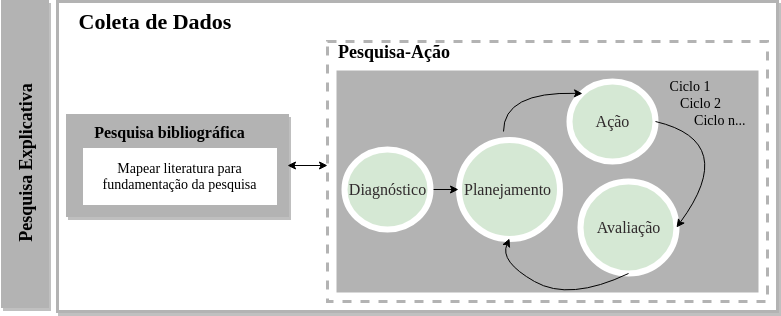
\includegraphics[width=12cm]{figuras/etapasPesquisaAcaoAdotadas.png}
          \caption{Etapas da Pesquisa-Ação adotadas. (Fonte: Elaborado pela Autora.)}
          \label{fig:etapasPesquisaAcaoAdotas}

        \end{figure}

\subsection{Técnicas de Coleta de Dados}

Durante a fase de Coleta de dados foram usadas as técnicas de observação, além de elaboração e uma futura aplicação de questionário para reconhecer o perfil de cada testador.

\section{Análise de Dados}

Após a fase Coleta de Dados, com a aplicação dos procedimentos de coleta de dados definidos, a fase seguinte será a de Análise dos Dados e Resultados, conforme o planejamento da pesquisa e apresentado na Figura \ref{fig:analiseDados}.

        \begin{figure}[H]
          \centering
          
\includegraphics[width=8cm]{figuras/analiseDados.png}
          \caption{Análise de Dados. (Fonte: Elaborado pela Autora.)}
          \label{fig:analiseDados}

        \end{figure}

\section{Resultados}

A fase de resultados corresponde à fase final deste trabalho, na qual os resultados obtidos com a execução do TCC2 serão apresentados. A Figura \ref{fig:resultados} apresenta a última fase do Plano Metodológico.

        \begin{figure}[H]
          \centering
          
\includegraphics[width=8cm]{figuras/resultados.png}
          \caption{Resultados. (Fonte: Elaborado pela Autora.)}
          \label{fig:resultados}

        \end{figure}


\section{Considerações Finais do Capítulo}

Considerando o foco deste trabalho em definir processos, principalmente, relacionados à atribuição de testes, a metodologia definida surgiu da necessidade de se experimentar um processo de atribuição de casos de testes de acordo com o perfil do testador. Desse modo, neste capítulo, apresentou-se o plano metodológico adotado para se atingir os objetivos desta pesquisa. 

No próximo capítulo apresenta-se a proposta deste trabalho, com as atividades já realizadas e as por realizar. Com especial detalhamento das atividades em cada estágio da Pesquisa-Ação.

% \del{acho que o cronograma está no capítulo seguinte, correto? rever aqui nas considerações finais o que realmente está nesse capítulo e o que será apresentado no próximo}.